\section{Methodology} \label{sec:methodology}


\subsection{Models Architecture}

\subsubsection{Probabilistic degradation model}

    This architecture, proposed in \cite{luo2022learning}, belongs to the implicit modelling blind super resolution methods. 
    Most methods in this category try to adaptively learn the degradation process via a deterministic model in order to avoid the domain gap between synthetic and test image.
    However, some degradations in real scenarios are stochastic and cannot be determined by the content of the image.
    These approach may fail to model the random factors and content-independent parts of degradations, which will limit the performance of the following SR models.
    In this architecture, the degradation D is assumed as a random variable, and a network learns its distribution by modeling the mapping from a priori random variable $z$ to D.
    Compared with previous deterministic degradation models, PDM could model more diverse degradations and generate HR-LR pairs that may better cover the various degradations of test images, and preventing the SR model from over-fitting to specific ones.

    Other degradation-learning-based SR methods have an assumption: the degradation is completely dependent on the content of the image.
    However, this may not hold in most cases.
    Some degradations are content independent and stochastic, such as random noises. 
    These random factors and content-independent parts of degradations could not be well modeled by these deterministic models. 
    A better assumption is that the degradation is subject to a distribution, which may be better modeled by a probabilistic model.
    
    The degradation is parametrized with two random variables, i.e., the blur kernel $k$ and random noise $\mathbf{n}$, by formulating the degradation process as the linear function from Eq. \ref{eq:2-degradation-equation}.
    It can be divided into two linear steps \cite{zhu2020unpaired}: 

    \begin{equation}
        \begin{aligned}
                I^{\text{LR}}_{\text{clean}} &= (I^{\text{HR}} * k) \downarrow_s \\
                \mathbf{I^{\text{LR}}} &= I^{\text{LR}}_{\text{clean}} + \mathbf{n}
        \end{aligned}
    \end{equation}
    
    Usually,the two steps are mutually independent, as the blur kernels are mainly dependent on the properties of the camera lens while the noises are mainly related to the properties of sensors. 
    Thus, the distribution of the degradation process can be represented as the product of the distribution of $k$ and $n$, which can be modeled by learning the mapping from a priori random variable $z$ to $k$ and $n$.


    \begin{equation}
        p_{D}(D) = p_{k,n}(k, n) = p_{k}(k)p_{n}(n).
    \end{equation}

    To model the distribution of the blur kernel k, we define a priori random variable $z_k$ which is subject to multi-dimensional normal distribution. 
    Then we use a generative module to learn the mapping from $z_k$ to k: 

    \begin{equation}
        k = \text{net}K(z_k), \quad z_k \sim \mathcal{N}(0,1),
    \end{equation}

    The spatially variant blur kernel is considered first. This implies that the blur kernel for each pixel of the image is different. In that case, we have

    \begin{equation}
        z_k \in \mathbb{R}^{f_k \times h \times w}, \quad k \in \mathbb{R}^{(k \times k) \times h \times w},
    \end{equation}

    where $f_k$ is the dimension of the normal distribution $z_k$, $k$ is the size of the blur kernel, $h$ and $w$ are the height and width of the image, respectively.
    Generally, the sizes of the convolutional weights  are set as 3 × 3, which indicates that the learned blur kernels are spatially correlated.
    Otherwise, if the spatial size of all convolutional weights is set as 1 × 1, the blur kernel could be approximated by a spatially invariant one, which is a special case of the spatially variant blur kernel with h = w = 1.
    This approximation simplifies the dimensions of the problem drastically and is an appropiate assumption if the crops used for training the model are small enough.
    A Softmax layer is added at the end of the network to guarantee that all elements of k sum to one.
    
    
    To model the distribution of the noise $n$, a vanilla generative module can also be used:

    \begin{equation}
        k = \text{net}N(z_n), \quad z_n \sim \mathcal{N}(0,1),
    \end{equation}

    \begin{equation}
        z_n \in \mathbb{R}^{f_n \times h \times w}, \quad n \in \mathbb{R}^{h \times w \times c},
    \end{equation}

    Where the height, width and number of channels of the image is noted as $h$, $w$ and $c$ respectively. 
    In this work, $c$ is always set to 1.

    In other methods \cite{plotz2017benchmarking}, the noise is modeled as a combination of shot and read noise. 
    It can be approximated as a heteroscedastic Gaussian distribution, which is dependent on the content of the image.

    \begin{equation}
        n \sim \mathcal{N}(0, \sigma_{\text{read}} + \sigma_{\text{shot}} \cdot I^{\text{LR}}_{\text{clean}}),
    \end{equation}

    This indicates that the noise is also related to the image content and the distribution of $n$ should be expressed as:


    \begin{equation}
        k = \text{net}N(z_n,I^{\text{LR}}_{\text{clean}}), \quad z_n \sim \mathcal{N}(0,1),
    \end{equation}

    \begin{figure}[h!]
        \centering
        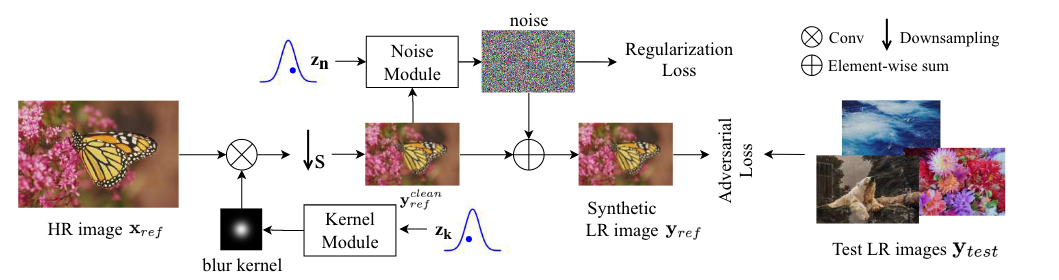
\includegraphics[width=\textwidth]{Includes/3-probabilistic-degradation-model.png}
        \caption{Schematic of the probabilistic degradation module.
                The discriminator is left out for a more intuitive description.}
        \label{fig:3-probabilistic-degradation-model}
    \end{figure}

    The probabilistic degradation model is optimized via adversarial training, which encourages the output of the generator to be similar with the test images \cite{bulat2018learn}.
    To avoid overly noisy images, a constraint to the noise level is added to the loss function via a regularization term. 
    A multiplication constant is also added to balance the magnitude of the two terms.

    \begin{equation}
        l_{\text{total}} = l_{\text{adversarial}} + 100 \|\mathbf{n}\|_2^2.
    \end{equation}

    This approach formulates the degradation process as a linear function, and the learned degradations can only impose a limited influence on the image content.
    In this way, it better decouples the degradations with image content and allows to focus on learning the degradations.
    This limitation eliminates the need of a guidance using a bicubically downscaled version of the HR image, as opposed to \cite{wei2020unsupervised} or \cite{bulat2018learn}.
    This guidance may be inappropriate, especially when the test images are heavily blurred.

    \begin{figure}[H]
        \centering
        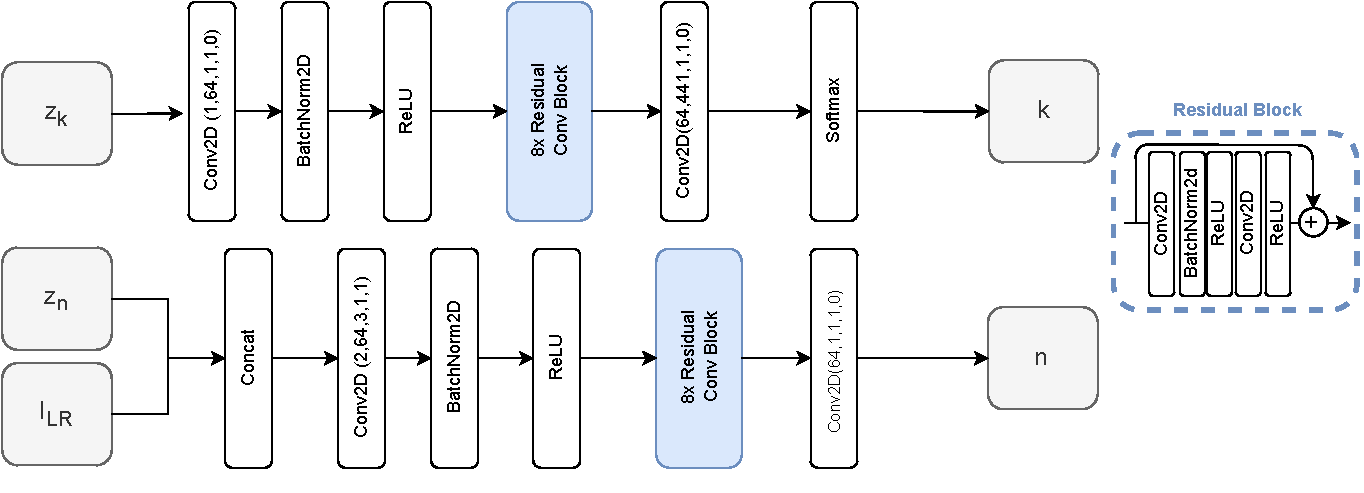
\includegraphics[width=\textwidth]{Includes/3-slim-gen-module.pdf}
        \caption{Schematic of the generative networks used in the kernel and noise module of the probabilistic degradation model.
        The parameters of the convolutional layers represent input channels, output channels, kernel size, stride and padding, respectively.
        The residual blocks use the same kernel size as the convolutional layers of each module. 
        In the noise module, the random vector $z_n$ is concatenated with $I_{\text{clean}}^{\text{LR}}$ before the first convolutional layer. }
        \label{fig:3-slim-gen-module}
    \end{figure}

    To discriminate the generated images from the test images, a PatchGAN discriminator is used \cite{isola2018imagetoimage}. This architecture assesses the structure of local image patches, allowing it to focus on high-frequency details of the image. This is particularly useful in the context of this work, where the generated images are expected to share a lot of information in the low frequencies of the domain and the differences with the test images are expected to be in the high frequencies. The architecture of the discriminator is shown in Fig. \ref{fig:3-slim-patchgan-module}.
    The network tries to classify if each N × N patch in an image is real or fake. The size of the patches depend mostly on the number of convolutional layers with stride 2 that are employed.  The discriminator outputs a matrix of values, where each value represents the probability that the corresponding patch is real. The final output is obtained by averaging the values in the matrix. The PatchGAN discriminator is trained to minimize a classification loss. 

    \begin{figure}[H]
        \centering
        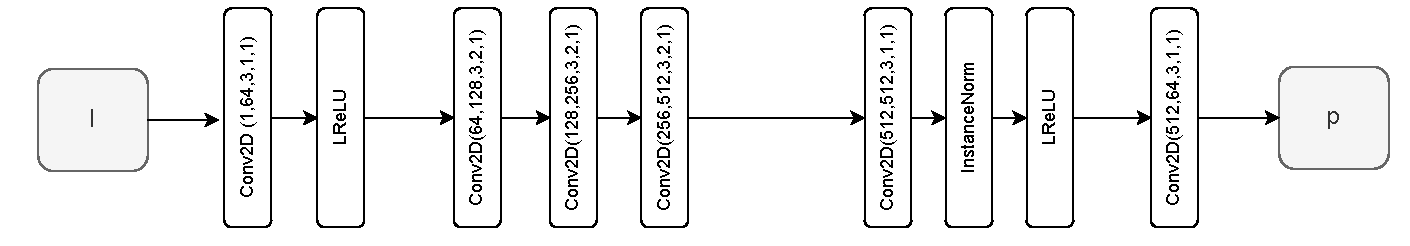
\includegraphics[width=\textwidth]{Includes/3-slim_patchGAN_architecture.pdf}
        \caption{Diagram of the PatchGAN discriminator.
                 The parameters of the convolutional layers represent input channels, output channels, kernel size, stride and padding, respectively. }
        \label{fig:3-slim-patchgan-module}
    \end{figure}

    
    The constrained nature of the probabilistic degradation model allows the possibility to train it simoultanously with a super resolution algorithm, as described in Fig. \ref{fig:3-GAN-degradation-model}.      
    In this way, PDM can be integrated with any SR model to form a unified framework for blind SR that can be trained in an end-to-end fashion, allowing for faster iterations.
    Other methods \cite{fritsche2019frequency} \cite{wei2020unsupervised} require that the training of the degradation model and the SR model in separate phases. They firstly train a degradation model and then use the trained degradation model to generate pairs and train the SR model.
    This two-step training method is time-consuming but necessary because the highly nonlinear degradation models used will produce undesirable results at the beginning of the training, which may mislead the optimization of the SR model.

    \begin{figure}[H]
        \centering
        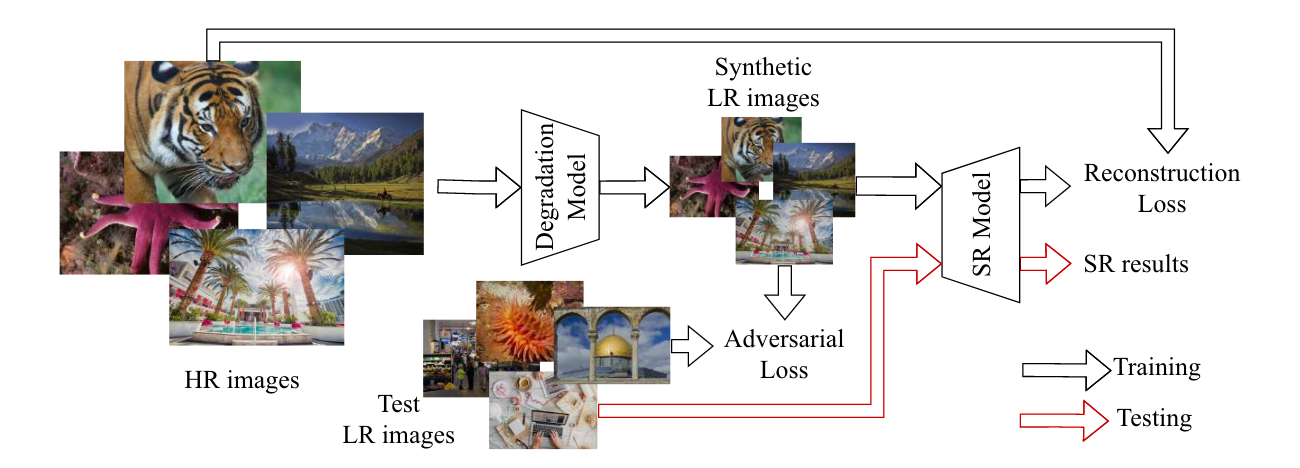
\includegraphics[width=\textwidth]{Includes/3-GAN-degradation-model.png}
        \caption{The probabilistic degradation model is used to encourage the degradation model to produce images in the same domain as the test LR images.
                After training, the SR model is directly used to super resolve the inputs.
                Source \cite{luo2022learning}.}
        \label{fig:3-GAN-degradation-model}
    \end{figure}

    This creates a very flexible framework for blind super resolution. 
    The only data requirement is a big enough unpaired dataset of LR and HR images and an optional smaller paired dataset for validation and early stopping of the model training.
    The biggest limitation of this approach is the one that degradation-learning-based methods have: the HR images (source domain) and the LR images (target domain) must be well defined and the model will not generalize a domain that is not the LR images. 
    Using this framework for general images is difficult, due to the variety of cameras and sensors, compression algorithms that play a part in the image distribution. However, this work is focused on 2 specific missions with a well defined degradation process, so this limitation is not a problem.


\subsubsection{SRResNet}

    
    To perform the super resolution task, the SRResNet architecture is used. This network has been used extensively in the literature and has proven to be a good baseline for SR. It can also be easily extended for multi-spectral super resolution, as in \cite{myself2023}. It uses a residual network architecture,in a post-upsampling framework based on sub-pixel convolution layers and a pixel based loss function.
    Introduced in 2017 \cite{ledig2017photorealistic}, SRResnet is the generator in the SRGAN architecture, which is a GAN-based super resolution method. The purpose of the GAN is to drive the reconstruction process towards the natural image manifold, producing more visually convincing solution. Additionally, a perceptual loss based on activation layers of a pre-trained VGG network \cite{simonyan2015deep} is incorporated to the training objective. As this work focuses on having super resolved images with high physical consistency and not on the perceptual superiority of the images, these two components are left out, and only the generator is going to be used. The architecture, with slight modifications, is detailed in Fig. \ref{fig:3-resnet-architecture}.

    First, features are extracted from the input using a convolutional layer with 64 filters and kernel size of 3, plus a ParametricReLU activation function.
    Before going through the core of the network, the feature map is reduced by half using a 1x1 convolutional layer.
    The core of the network is composed of 5 residual blocks, consisting of two convolutional layers, followed by batch-normalization layers and ParametricReLU activation functions. 
    The convolutional layers have 3x3 kernels and 64 feature maps. 
    To increase the resolution of the input image, two trained sub-pixel convolution layers are used.

    \begin{figure}[H]
        \centering
        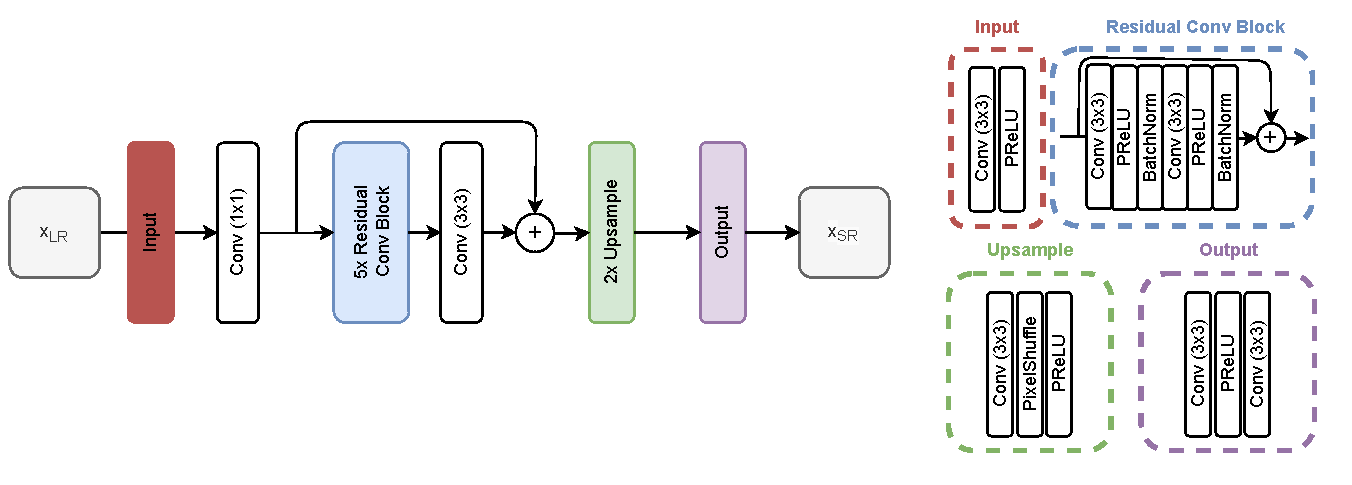
\includegraphics[width=1\textwidth]{includes/3-srresnet-architecture.pdf}
        \caption{ Modified SRResNet architecture. $X_{LR}$ represents the low resolution input image, $X_{SR}$ the super resolved image, which is then compared to the ground truth $X_{HR}$.}
        \label{fig:3-resnet-architecture}
     \end{figure}
    
    \subsection{Baseline Degradation model} \label{subsec:baseline_degradation_model}

        As stated in \ref{subsec:domaingap}, early super-resolution methods commonly generated high-resolution (HR) to low-resolution (LR) samples using predefined degradation techniques, with bicubic downsampling being the most used setting \cite{zhang2018residual}.
        This kind of synthetic data, while easy to obtain, often results in a domain gap problem, where the data used for training and assessing the model do not come from the same distribution as real data.
        This gap usually leads to performance drops when the models implemented in production environments.
        A possible solution is to synthesize samples with a stochastic degradation model, which includes a set of multiple blurring kernels and several random noises configurations that convert scenes from an HR mission into LR versions, as if they were taken using FOREST-2.
        The larger degradation space grant these models better generalization capabilities and let experts be part of the kernel definition process, based on prior knowledge of the degradation process.
        Unfortunately, the variety of predefined degradation's is still limited and still fail in most applications.

        A degradation model like this one will be used as a baseline for this work.
        

        \subsubsection{Blurring Kernel}

        In the literature, the kernel of the degradation process is usually modelled as a fixed isotropic gaussian kernel, with a parameter $\sigma$ that depends on the scale factor of the super resolution process.
        To provide more variability to it to each dataset pair, the parameters of the blurring kernel that determine it's width in both axis, $\sigma_x$ and $\sigma_y$, are sampled from a normal distribution with a determined mean and standard deviation. Fig. \ref{fig:4-degradation_kernels} shows some examples of kernels generated using this method, in the upper row, both distributions have a similar mean and distribution, resulting fairly isotropic kernels. In the lower row, the mean of the x axis is much higher than the variance of the x axis, resulting in highly anisotropic kernels. The effects of these kernels on the HR-LR generation are shown in Fig. \ref{fig:4-degradation-kernel-examples}.



        \begin{figure}[H]
                \centering
                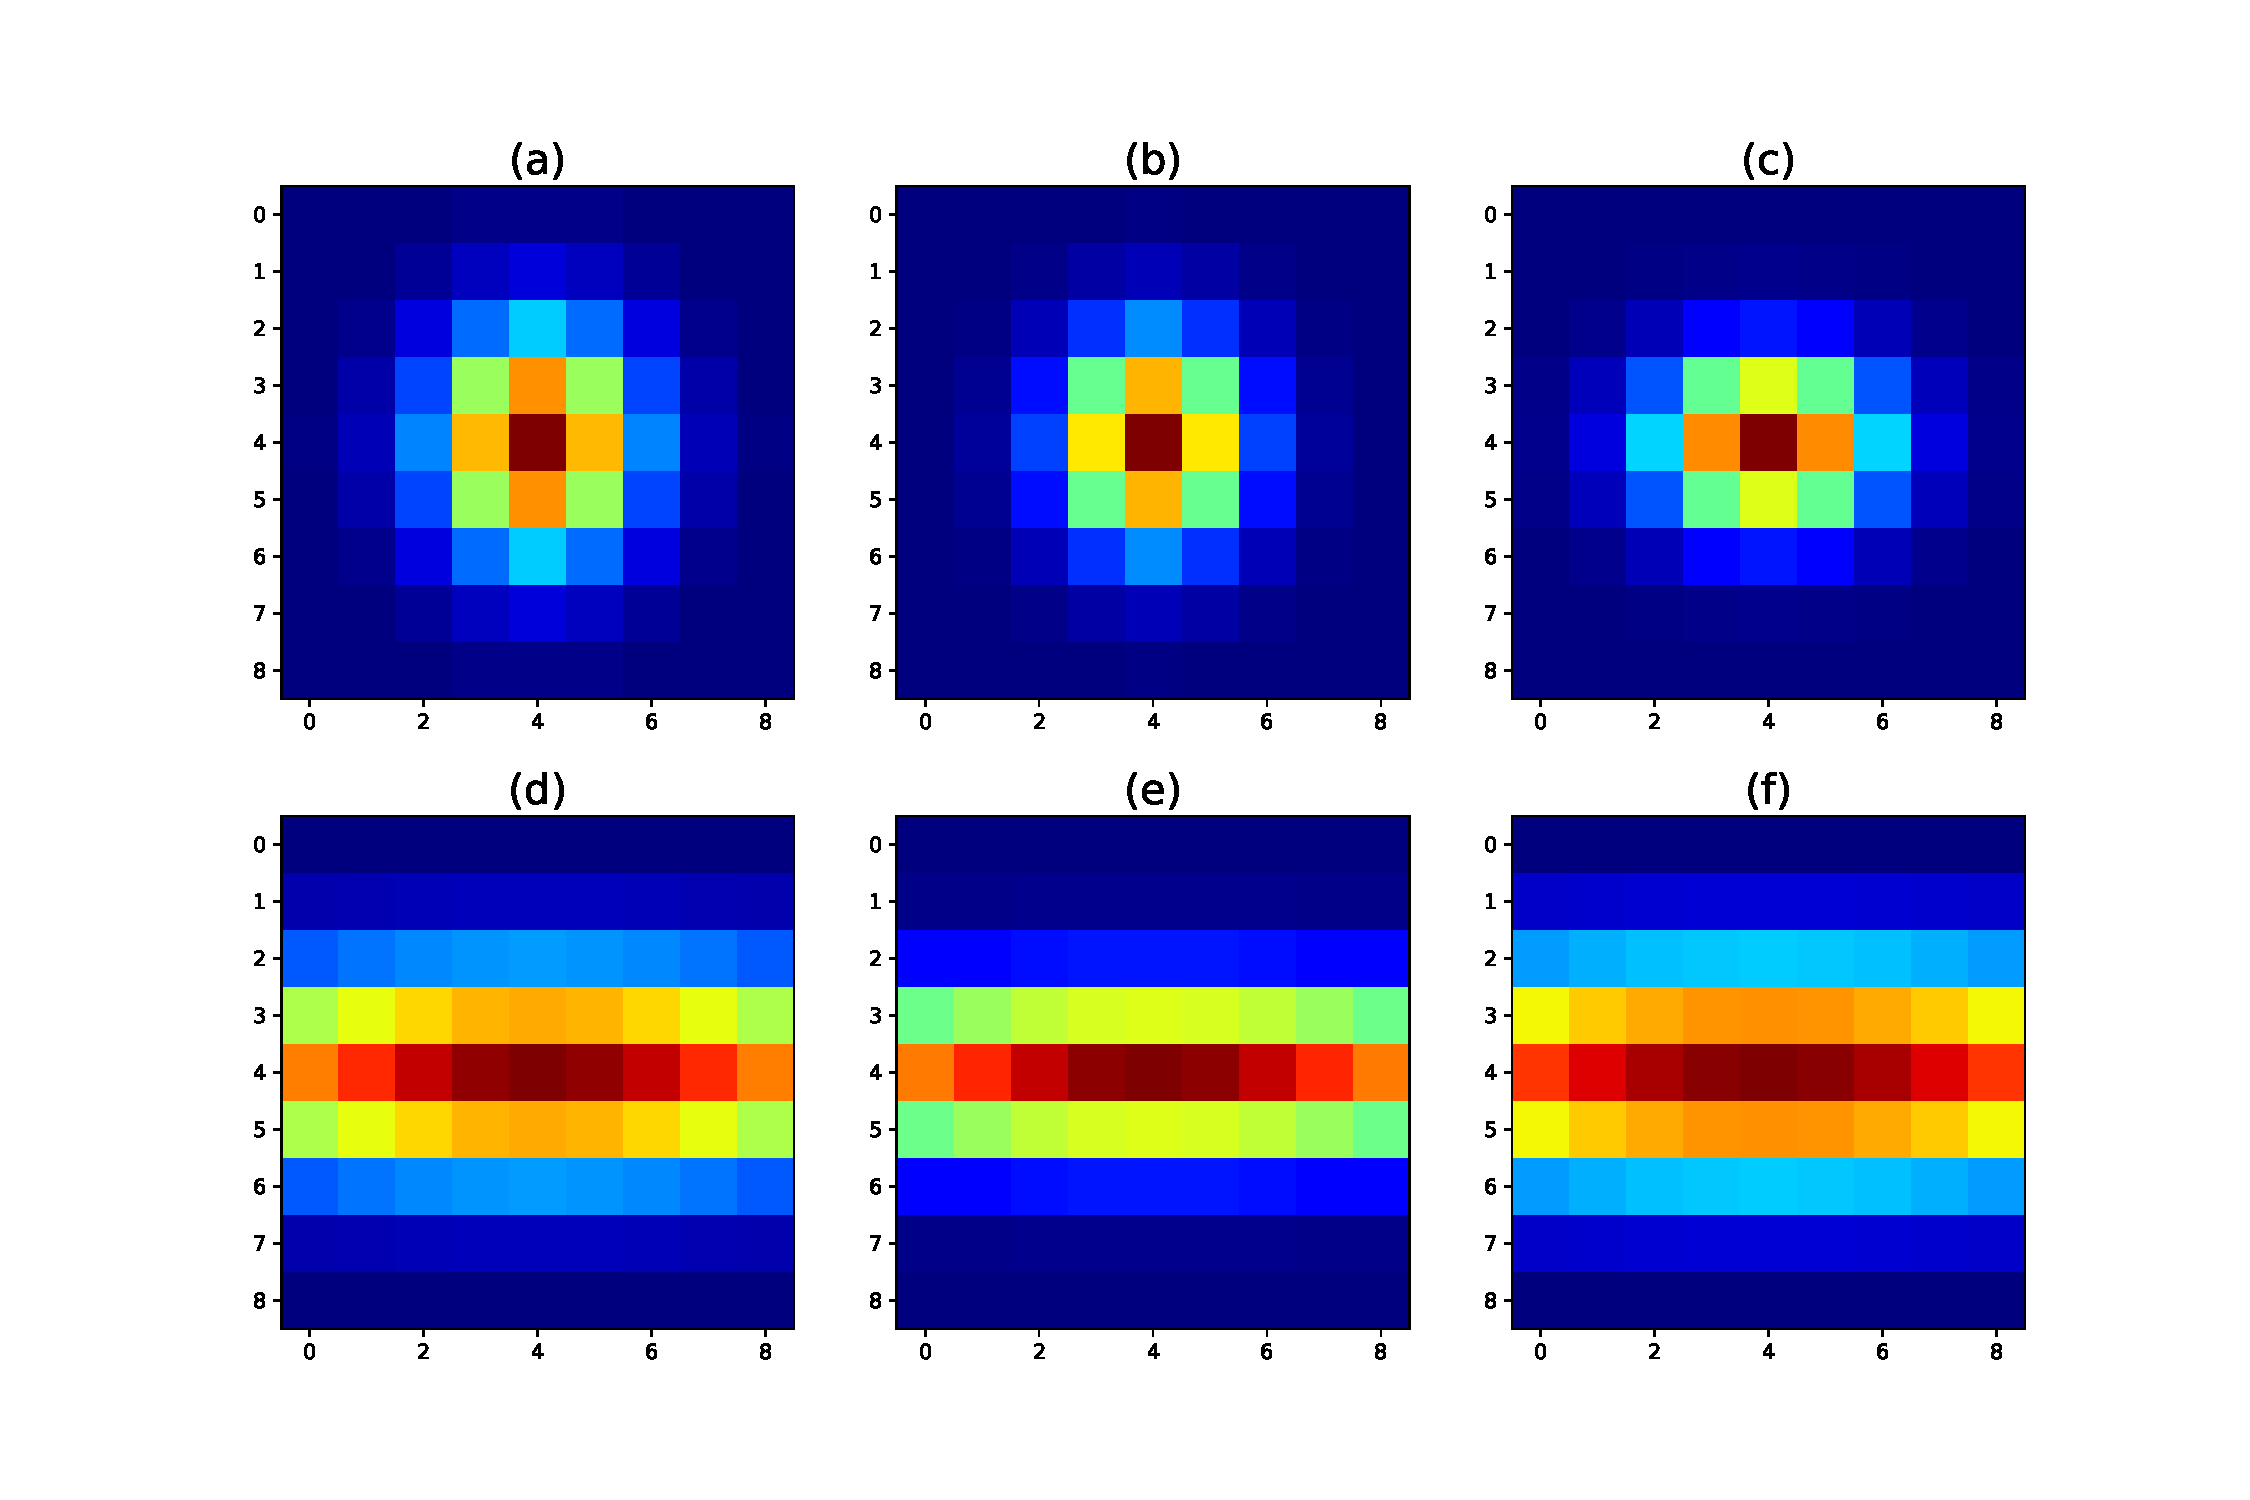
\includegraphics[width=\linewidth]{Includes/4-degradation_kernels.pdf}
                \caption{Example of kernels used in a stochastic degradation model. (a),(b) and (c) are generated using a symmetric variance on the x and y axis. (d) (e) and (f) are generated using an asymmetric variances, resulting in much more anisotropic kernels.}
                \label{fig:4-degradation_kernels}
            \end{figure}

        \begin{figure}[H]
                \centering
                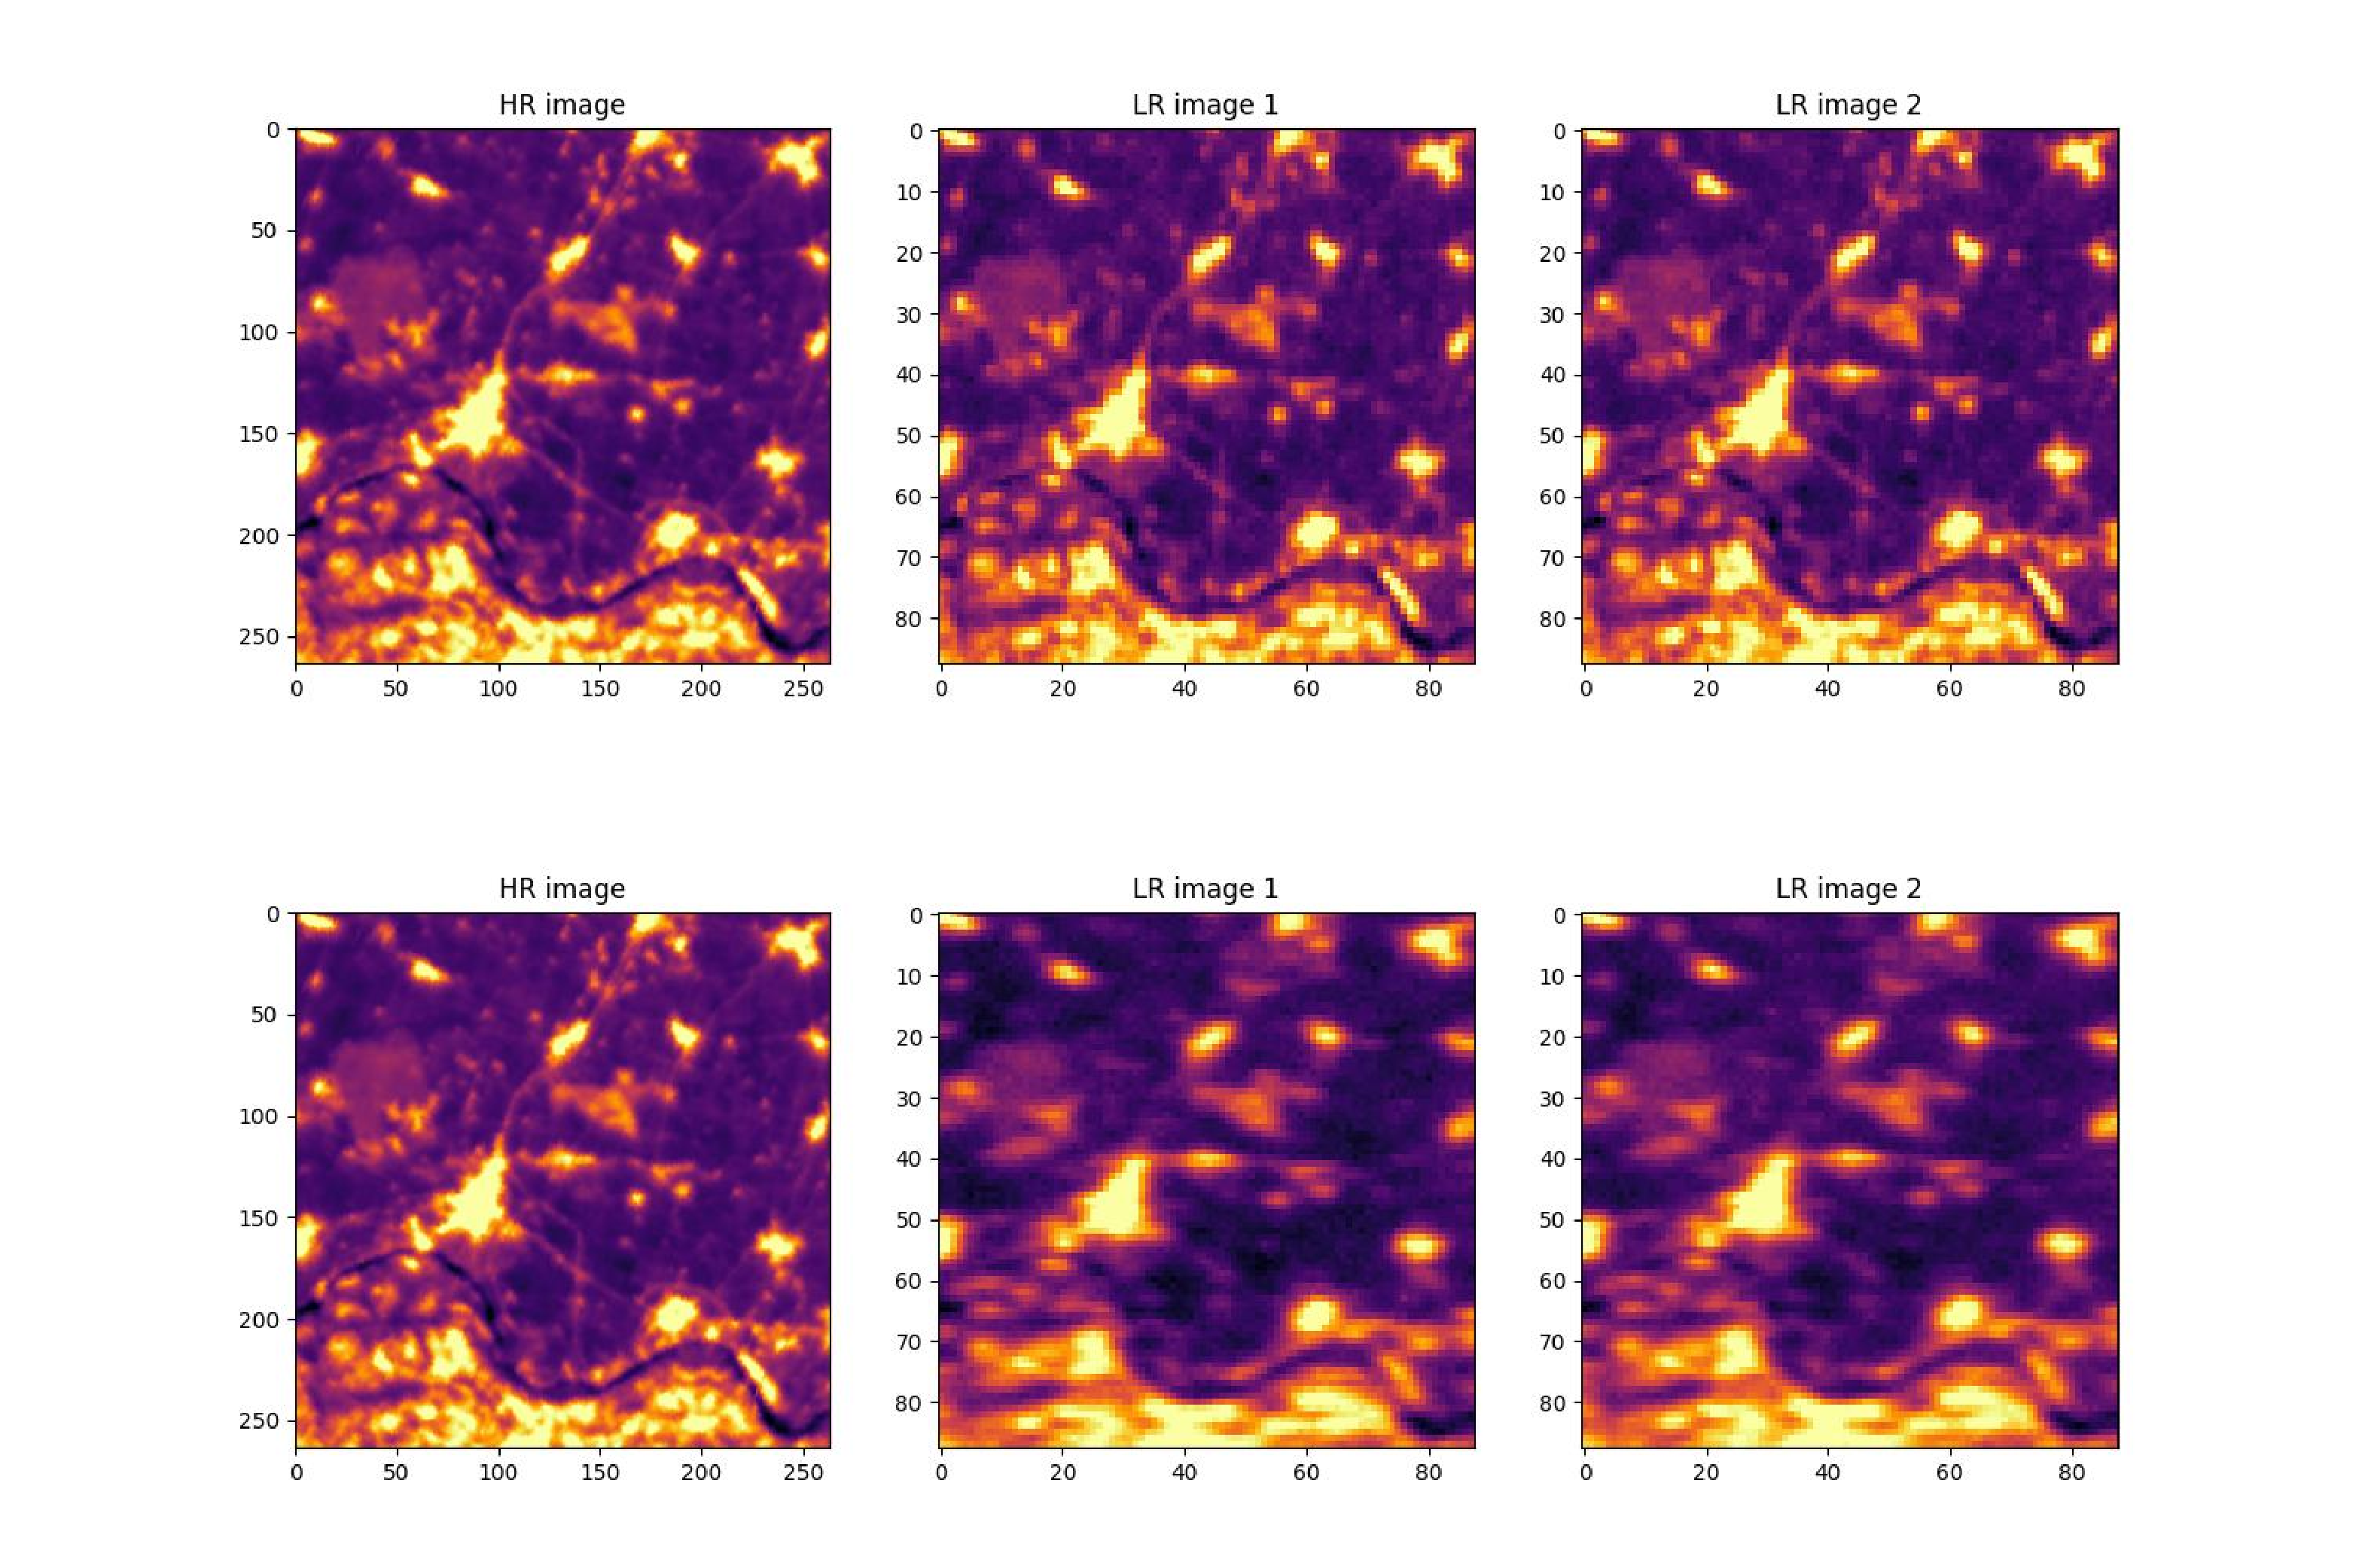
\includegraphics[width=\linewidth]{Includes/4-degradation-kernel-examples.pdf}
                \caption{Effects of different blurring kernels on the HR-LR generation. The upper row contains images generated using blurring kernels with symmetric distributions. The lower rows contains images generated using asymmetric distributions for the variances, resulting in highly anisotropic kernels.}
                \label{fig:4-degradation-kernel-examples}
            \end{figure}
            
        \subsubsection{Radiometric error correction}

        FOREST-2 radiometric accuracy is 1K at 300K.
        Other missions report lower nominal radiometric accuracies, such as the case of ECOSTRESS instrument sheet \cite{ECOSTRESS2023INSTRUMENT} which is 0.5K at 300K.
        This difference in accuracy should be taken into account. To align these accuracies, we first calculate the additional error required using the following equation:

        \begin{equation}
            e_{\text{forest}} = \sqrt{e_{\text{eco}}^2 + e_{\text{extra}}^2} 
            \label{eq:4-radiometric-error-correction}
        \end{equation}
        
        where $e_{\text{eco}}$ is the ECOSTRESS error, and $ e_{\text{extra}}$ is the additional error required for FOREST-2.
        
        Using the above equation, we find that an additional radiometric error of approximately 0.8660K is needed. The next step involves converting this extra error into a radiance value. This requires calculating the derivative of the Planck equation at 300K, which is done numerically as follows:
        
        \begin{equation}
            \frac{\partial B}{\partial T} = \frac{B(\lambda, T + \delta T) - B(\lambda, T)}{\delta T}
            \label{eq:4-planck-derivative}
        \end{equation}  
        
        By multiplying the results of equations \ref{eq:4-radiometric-error-correction} and \ref{eq:4-planck-derivative}, we can obtain the radiance error for both FOREST LWIR bands. The additional radiance errors for LWIR1 and LWIR2 bands are found to be \(1.5472 \times 10^{-1}\) W/sr/m\(^2\)/\(\mu m\) and \(1.1444 \times 10^{-1}\) W/sr/m\(^2\)/\(\mu m\), respectively.

        The difference in radiances will be split into two components. On one side, the cold Bias represents a systematic error in the measurement, this error acknowledges discrepancies that can be attributed to sensor calibration and atmospheric conditions. On the other side, the random noise accounts for unpredictable fluctuations in the measurement process. It could be due to a variety of sources like electronic noise in the sensor, random atmospheric disturbances, or other stochastic factors. As the extent of each component is not known and to give more variability to this basic degradation model, a random factor $\phi \in [0,1] $ is introduced so that:

        \begin{equation}
        \begin{aligned}
            \varepsilon_{\text{final}} &= (1 - \phi) \times \varepsilon_{\text{radiance}} + \phi \times \eta \times \varepsilon_{\text{radiance}} \\
            \eta & \sim \mathcal{N} (0,1)
        \end{aligned}
        \end{equation}    

        The effects of the error correction is shown in Fig. \ref{fig:4-radiometric_noise_example}. As the target radiometric error increases with respect to ECOSTRESS scenes, the loss of information is more noticeable.


        \begin{figure}[h!]
            \centering
            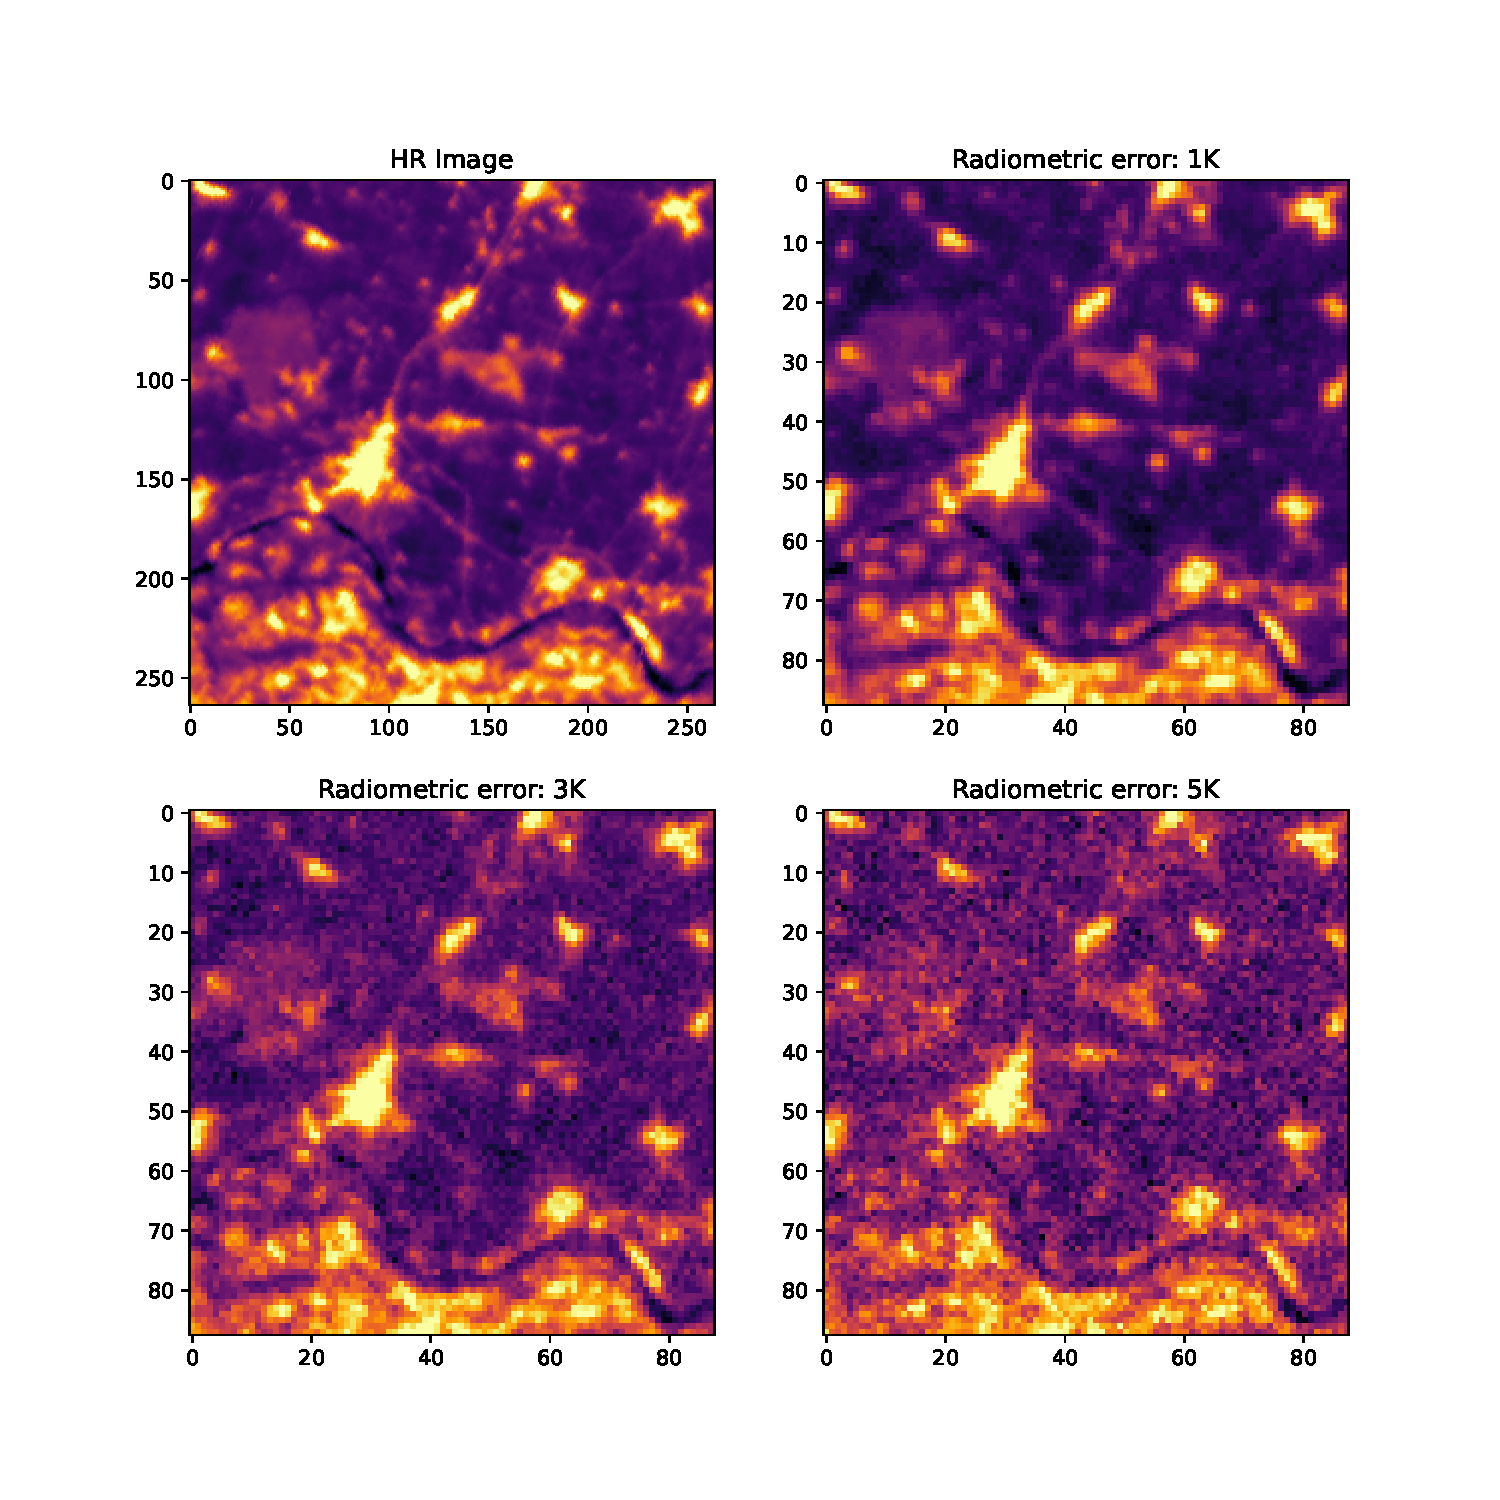
\includegraphics[width=\textwidth]{Includes/4-radiometric_noise_example.pdf}
            \caption{Effects of increasing radiometric error on the HR-LR generation.}
            \label{fig:4-radiometric_noise_example}
        \end{figure}
        
    

    \subsection{Signal-to-Noise Ratio (SNR)}

        To quantify how much a signal is corrupted by noise, the Signal-to-Noise Ratio (SNR) is used used. It is defined as the ratio of signal power to the noise power and is usually expressed in decibels (dB). Mathematically, the SNR is often defined as:

        \[ \text{SNR} = 10 \log_{10} \left( \frac{P_{signal}}{P_{noise}} \right) \]

        Where $P_signal$ and $P_noise$ represent the power of the signal and the noise tensors, calculated as the sum of their squared elements.
        A higher SNR indicates a clearer and more distinguishable signal in comparison to the noise. In the context of this work, it will be used to assess the power of the noise introduced by the probabilistic degradation model, compared to the clean image.

    \subsection{Referenced image quality metrics}

        When the ground truth high resolution image is available, the performance of a super-resolution algorithm can be evaluated using a variety of metrics. 
        These metrics can be divided into two categories: pixel-based and perceptual-based.
        Pixel-based metrics are based on the pixel-wise comparison between the generated image and the ground truth. 
        Perceptual-based metrics, on the other hand, are based on the perceptual similarity between the generated image and the ground truth. 
        These metrics are build using a pre-trained deep neural network, which is usually trained on a large dataset of images.
        The following sections will describe the most commonly used metrics in the literature.

        \subsubsection{pixel-wise losses}

            The $L_1$ and $L_2$ losses are the most commonly used pixel-based metrics in the literature. 
            Additionally, they are usually used as the loss function that drives the super resolution network gradients during training. 
            In a general form, the $L_1$ and $L_2$ losses are defined as follows:

            \begin{equation}
                \mathcal{L}_{L_k} = \frac{1}{N} \sum_{i=1}^{N} |y_i - \hat{y}_i|^k
            \end{equation}

            Where $y_i$ and $\hat{y}_i$ are the ground truth and the super resolved image, respectively, and $k$ is the exponent of the loss function. 
            The $L_2$ loss weights high-value differences higher than low-value differences due to the exponent of 2. 
            This generates overly smooth for low values and a lot of variability in high values. 
            For that reason, it is more common to see the $L_1$ loss being used in the literature and it will be employed in this experiment .

        \subsubsection{Peak Signal-to-Noise Ratio (PSNR)}

         
            Peak Signal-to-Noise Ratio (PSNR) measures the magnitude of the error, compared relatively with the reference image. It is usually used to quantify the amount of error or noise introduced during the image reconstruction process.
            
            PSNR is calculated by first computing the Mean Squared Error (MSE) or $\mathcal{L}_2$ loss between an image and the reference, and then taking the logarithmic ratio of the maximum possible pixel value squared. The PSNR value is usually expressed in decibels (dB).
            
            The formula for PSNR is:
            
            \begin{equation}
            PSNR = 10 \cdot \log_{10} \left( \frac{I_{MAX}^{2}}{\mathcal{L}_2} \right)
            \end{equation}
            
            where $I_{MAX}$ is the maximum possible pixel value of the reference image, and $\mathcal{L}_2$ is the mean squared error between the image and the reference.
            
            A higher PSNR value indicates better quality of the super-resolved image, as it signifies a lower level of noise or error. However, it's worth noting that it may not always align with human perceptual evaluations of image quality, as it focuses on physical consistency.

        \subsubsection{Structural Similarity Index (SSIM)}

            
        Structural Similarity Index Measure (SSIM) takes into consideration changes in structural information, luminance, and contrast. By doing that, it manages to reflect better the perceived changes in noise level and contrast.
        The SSIM index is calculated by dividing the image into windows of a certain size, and then comparing corresponding windows in the reference and target images. The SSIM index for a pair of windows, say $x$ and $y$, is given by:
        
        \begin{equation}
            SSIM(x, y) = \frac{(2\mu_x\mu_y + c_1)(2\sigma_{xy} + c_2)}{(\mu_x^2 + \mu_y^2 + c_1)(\sigma_x^2 + \sigma_y^2 + c_2)}
        \end{equation}
        
        where $\mu_x$ and $\mu_y$ are the average pixel values, $\sigma_x^2$ and $\sigma_y^2$ are the variances, $\sigma_{xy}$ is the covariance of $x$ and $y$, and $c_1, c_2$ are small constants to avoid division by zero.
        The final SSIM score for the images is calculated by averaging the SSIM indices of all windows. An SSIM score of 1 indicates a perfect structural match between the two images, whereas a score of 0 indicates no structural similarities.

        \subsubsection{Learned perceptual image patch similarity (LPIPS)}

        LPIPS is a perceptual metric that leverages deep learning to compute perceptual differences between images. Specifically, it uses the activations of a pre-trained convolutional neural network (in this case, VGG \cite{VGGnet} ) to extract perceptual features from the images. 
        Then, it calculates the Euclidean distance between these feature vectors to measure the perceptual difference.
        This measure has gained popularity in SR tasks due to its high correlation with human judgments of visual similarity.
        
        The LPIPS score is given by:
        
        \begin{equation}
        LPIPS(I, I') = \sqrt{\sum_{i=1}^{N} w_i\|f_i(I)-f_i(I')\|^2}
        \end{equation}
        
        where $I$ and $I'$ are the images being compared, $f_i(I)$ denotes the $i$-th layer activation when image $I$ is input to the pre-trained network, $N$ is the number of layers considered, and $w_i$ is the learned weight for the $i$-th layer.
        
        A lower LPIPS score indicates a lower distance between the feature vectors, and thus a greater perceptual similarity between the two images. 
        Due to the fact that in this work we are interested in the physical consistency of the super-resolved images, 
        this metric will be shown but will not drive any decision during the training process.
        

        \subsubsection{Adjusting measures to a slight translations in the SR process.}
    
            In order to calculate the losses and performance metrics, the generated test images (SR) are compared against the ground truth high resolution images (HR).
            Additional changes should be introduced in a MISR environment \cite{martens2019superresolution}.
            First, minor shifts on the contents of the pixels are expected and the metrics should have some tolerance to small pixel-translations in the high-resolution space by evaluating on a sliding cropped image. 
            That means, looking for a displacement of SR by at most d pixels in each direction that minimizes the error. 
            An example of how this is applied in a loss that needs to be minimized can be found in Eq. \ref{eq:4_adjusted_metrics}
    
            \begin{equation}
               \mathcal{L}^* ( I^{HR}, I^{LR}, d) = \min_{u,v \in [0,2d]} \mathcal{L} ( I^{HR}_{u,v}, I^{SR}_{u,v})
            \label{eq:4_adjusted_metrics}
            \end{equation}
    
            Additionally, commonly used metrics punish biases as much as noise in the reconstruction.
            For example, if $I^{SR} = I^{HR} + \epsilon$, where $\epsilon$ is a constant bias, a perfect reconstruction of $I^{SR}$ is possible if $\epsilon$ is known. 
            A quality metric should award a high score in super-resolutions with this characteristics in comparison to the introduction of noise and information loss. Metrics like L2/L1 losses and PSNR do the exact opposite and should have a bias compensation like the following: 
    
            \begin{equation}
                \begin{aligned}
                    \mathcal{L}^* ( I^{HR}, I^{LR}, d) = \min_{u,v \in [0,2d]} \mathcal{L} ( I^{HR}_{u,v}, (I^{SR}_{u,v}+b)) \\
                    b = \frac{1}{(W - d)(H - d)} \sum_{x,y} \left( I^{HR}_{u,v} - I^{SR}_{u,v} \right)
               \end{aligned}
            \end{equation}
    
            \noindent where $W$ and $H$ represent the width and height of the image, respectively.
    

    \subsection{Non-referenced Image quality metrics}

    No-Reference Image Quality Assessment (NR-IQA) aims to develop methods to measure image quality in alignment with human perception without the need for a high-quality reference image. 
    Most of them are based on two steps: feature extraction and quality prediction using a regression module. 
    They rely on the assumption that natural images share certain statistical information and that any distorsion may alter these statistics \cite{niqe}.
    The results from any image an arbitrary image is compared to a default model trained on a large dataset of natural scenes. 
    The difference  between them is used to predict the quality of the image.
    In the last years, researchers relied on deep learning to perform the two steps in a single model. 
    The workflow of these models is shown in Fig. \ref{fig:4-nr-iqa-workflow}.

    \begin{figure}[h!]
        \centering
        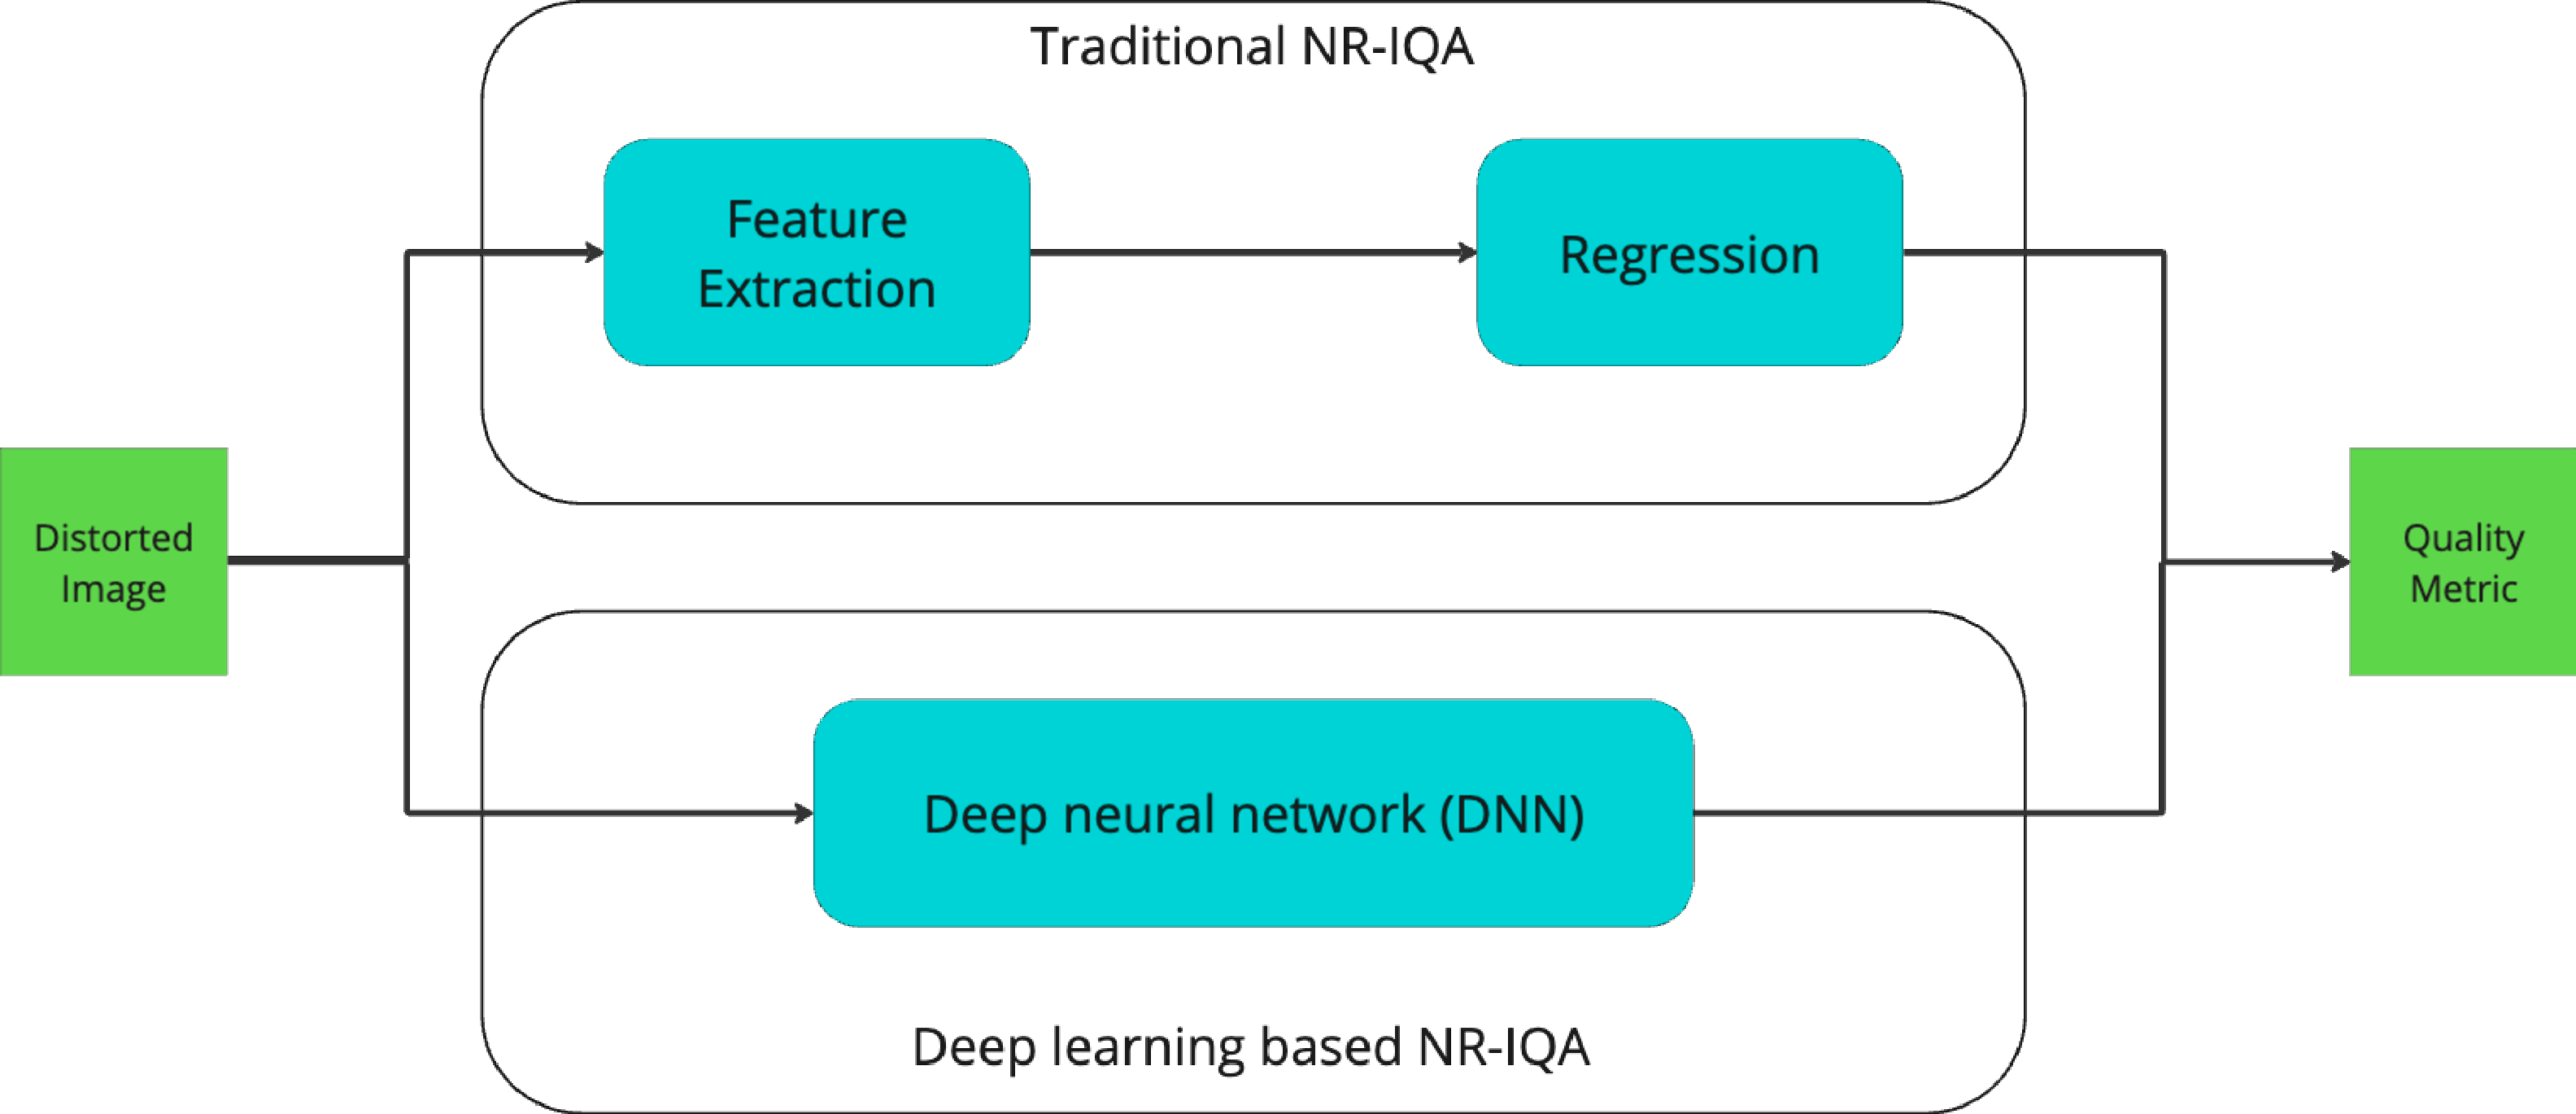
\includegraphics[scale=0.25]{Includes/3-NR-IQA.pdf}
        \caption{Workflow of a NR-IQA model.}
        \label{fig:4-nr-iqa-workflow}
    \end{figure}


        

        \subsubsection{Naturalness Image Quality Evaluator (NIQE)}

        
            The Naturalness Image Quality Evaluator (NIQE) \cite{niqe} is a no-reference image quality assessment metric that quantifies the perceptual quality of images based on their naturalness.
            NIQE operates on the principle that pristine natural images exhibit specific statistical properties that can be quantified to establish a benchmark for quality assessment. 
            NIQE employs a model based on a multivariate Gaussian distribution, characterized by a mean vector and covariance matrix, to represent the statistical attributes of a natural image's visual patterns.
            To assess the quality of an image, NIQE extracts a corresponding set of features and evaluates their deviation from this statistical model using the Mahalanobis distance.
            This distance measures the divergence of the image's features from those typical of high-quality natural images.
            A lower value suggests that the image closely resembles the statistical properties of natural images, indicating higher perceived quality.
            
            However, NIQE provides a measure of image quality that aligns with the naturalness of human visual perception, and is not able to quantify the physical consistency of a generated image.

        \subsubsection{Blind/Referenceless Image Spatial Quality Evaluator (BRISQUE)}

            Similar to NIQE, the Blind/Referenceless Image Spatial Quality Evaluator (BRISQUE) \cite{mittal2012} operates on the premise that natural images possess certain statistical properties which are altered in the presence of distortions. 
            
            It operates by quantifying deviations from the statistical regularities observed in natural images, primarily using locally normalized luminance coefficients. 
            Following this, a spatial domain model is utilized to calculate a set of features. 
            These features, derived from the locally normalized luminance coefficients, are designed to capture the loss of "naturalness" due to the presence of distortions.
            These extracted features are fed into a Support Vector Regression (SVR) that was pretrained with a set of images with known quality ratings, to predict the quality score of the image.
            
            A lower BRISQUE score is indicative of better quality, implying that the image has better quality score in the pre-trained model. The main difference between BRISQUE and NIQE is that BRISQUE uses a Support Vector Regression (SVR) model and predicts directly the quality score, while NIQE calculates the distance between the multivariate Gaussian distribution model of the image and the one from the specific dataset where the evaluator was pre-trained.




        \subsubsection{Frequency Domain Analysis} \label{subsubsec:frequency_domain_analysis}
        
        The Fourier transform is widely used to analyze the frequency content in signals.
        It can be applied to multidimensional signals such as images, where the spatial variations of pixel-intensities have a unique representation in the frequency domain. 
        Super-resolutions objective is to reconstruct missing high frequency components from a downscaled image.
        The expectation of a good SR algorithm is to amplify the high frequency components compared to a baseline like bicubic interpolation, while keeping noise at bay.
        The Fourier components provide global information about the image, as opposed to local information represented by pixel values in the spatial domain \cite{fuoli2021fourier}. 
        Using the Fast Fourier Transform (FFT), we convert the pixel intensity values of super-resolved images into a spectrum where each point represents a specific frequency contained in the spatial domain.
        The FFT is shifted so that the zero-frequency component is at the center of the spectrum. 
        The resulting magnitude, after applying a logarithmic transformation, reveals the energy distribution across various frequencies.
        This is visualized in grayscale, where the intensity corresponds to the amplitude of the frequency components.
        
        A radial profile of the FFT magnitude provides insights into how different spatial frequencies contribute to the image content in the vertical and horizontal direction.
        The radial profile is a function of the average intensity of frequencies at a given radius from the center of the Fourier transform.
        The average of the FFT magnitude is calculated for concentric circles of increasing radii, capturing a statistic of the frequency components in every direction.
        This metric serves as a benchmark for evaluating the performance of SR techniques against traditional interpolation methods such as bicubic interpolation.
        
        Spatial frequency within an image context refers to the periodicity of the intensity variation over spatial dimensions, typically quantified in cycles per pixel. The central region of the frequency domain, after the shift operation, denotes the zero frequency. In contrast, the extremities of the domain delineate the highest frequencies, constrained by the image's discrete sampling rate.
        To quantitatively interpret these spatial frequencies, a radial-to-frequency mapping is necessary. This mapping accounts for the Nyquist frequency, which is delineated as half the sampling rate of the discrete imaging grid and acts as a threshold to prevent frequency aliasing.
        The conversion from a given radius in the FFT output to the corresponding spatial frequency is formalized as:

        \begin{equation}
            f(r) = \frac{r}{\frac{N}{2}} \cdot f_{\text{Nyquist}},
        \end{equation}

        where \( f(r) \) signifies the spatial frequency associated with radius \( r \), \( N \) represents the FFT image dimension, assuming a square configuration, and \( f_{\text{Nyquist}} \) the Nyquist frequency, which is 0.5 cycles per pixel in this case.

        \begin{figure}[H]
            \centering
            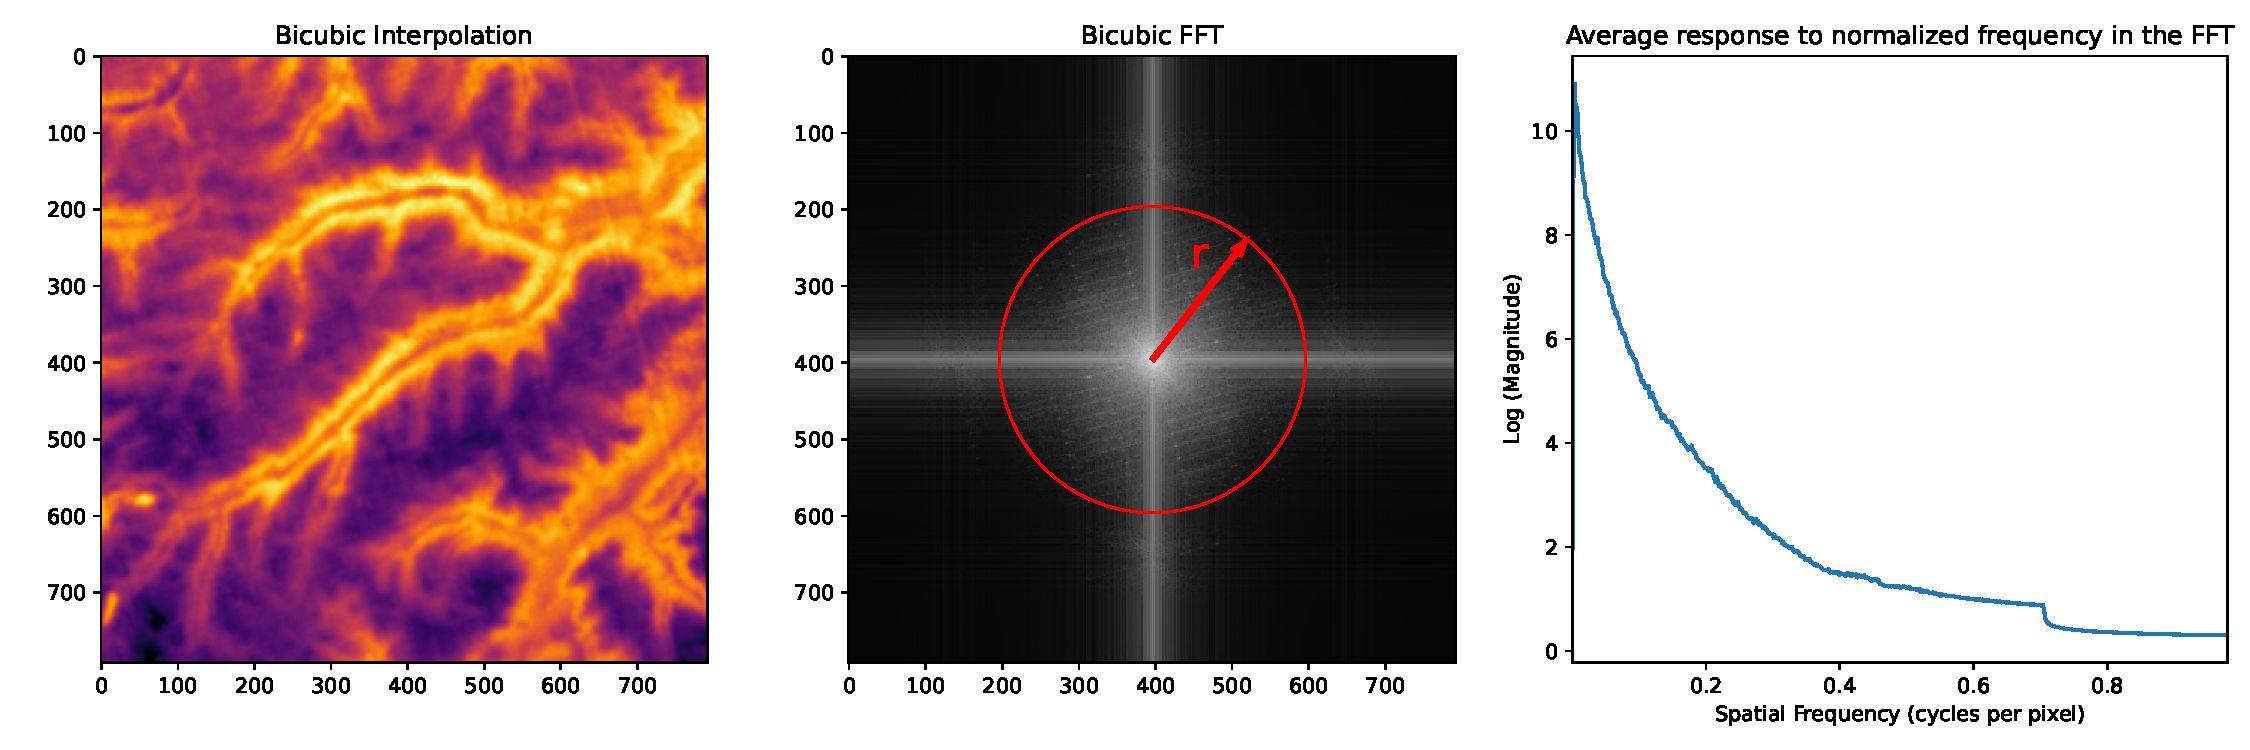
\includegraphics[width=\linewidth]{Includes/4-frequency-analysis.pdf}
            \caption{Steps of the frequency domain analysis. The Center image shows the log magnitude of the shifted FFT of a bicubic upsampled FOREST scene and an example of a radial profile, the average of all the points that have the same $r$ is calculated. The right image displays the log magnitude obtained for every radial profile, translated into spatial frequency.  }
            \label{fig:4-frequency-analysis}
        \end{figure}

        Through FFT a depiction of the amplification or attenuation of frequencies attributable to the SR techniques. 
        Analyzing these profiles displays the ability of SR models for detail enhancement. 
        However, it is important to note that this method does not account artifacts generated by the SR, and should be used in combination to other supervised metrics.

        \subsubsection{Gradient Distribution analysis}


        An alternative way of analyzing super-resolution results is by looking at the gradients of the images. 
        HR images are sharper and thus each pixel, on average, has higher gradients magnitude with respect to both directions than their LR counterparts.
        A super-resolution algorithm should increase the sharpness of the edges, resulting in a gradient distribution that aligns more closely with that of the genuine HR image.
        An approximation of the gradients can be estimated by doing 2d convolutions between an image and the so called Sobel kernels displayed in Eq. \ref{eq:4-sobel-operators} \cite{Sobel1990AnI3}.
        These kernels are designed to respond maximally to edges running vertically and horizontally relative to the pixel grid.
        
        \begin{equation}
            \begin{array}{ccc}
            \hat{G}_x = \begin{bmatrix}
            -1 & 0 & +1 \\
            -2 & 0 & +2 \\
            -1 & 0 & +1
            \end{bmatrix}
            &
            \quad
            &
            \hat{G}_y = \begin{bmatrix}
            +1 & +2 & +1 \\
             0 &  0 &  0 \\
            -1 & -2 & -1
            \end{bmatrix}
            \end{array}
            \label{eq:4-sobel-operators}
        \end{equation}
    
         The kernels can be applied separately to the input image to produce the component of the gradient in each orientation $G_x$ and $G_y$. The magnitude of the gradient  is given by: 
         \begin{equation}
             |G| = \sqrt{G_x^2 + G_y^2}
             \label{eq:4-gradient_magnitude}
         \end{equation}

         The gradient magnitude histograms of the results of different super-resolution algorithms will be assessed, there by quantifying the enhancement in edge sharpness.
         This histogram provide insights into the frequency and intensity of the edges within an image.
         A better SR model should demonstrate a histogram with higher frequencies of larger gradient magnitudes, indicating sharper edges.
         However, it is important to note that this analysis is unsupervised and disregards the effect of noise and artifacts introduced during the super-resolution process and should be considered in combination with other supervised metrics like PSNR.

         \begin{figure}[H]
             \centering
             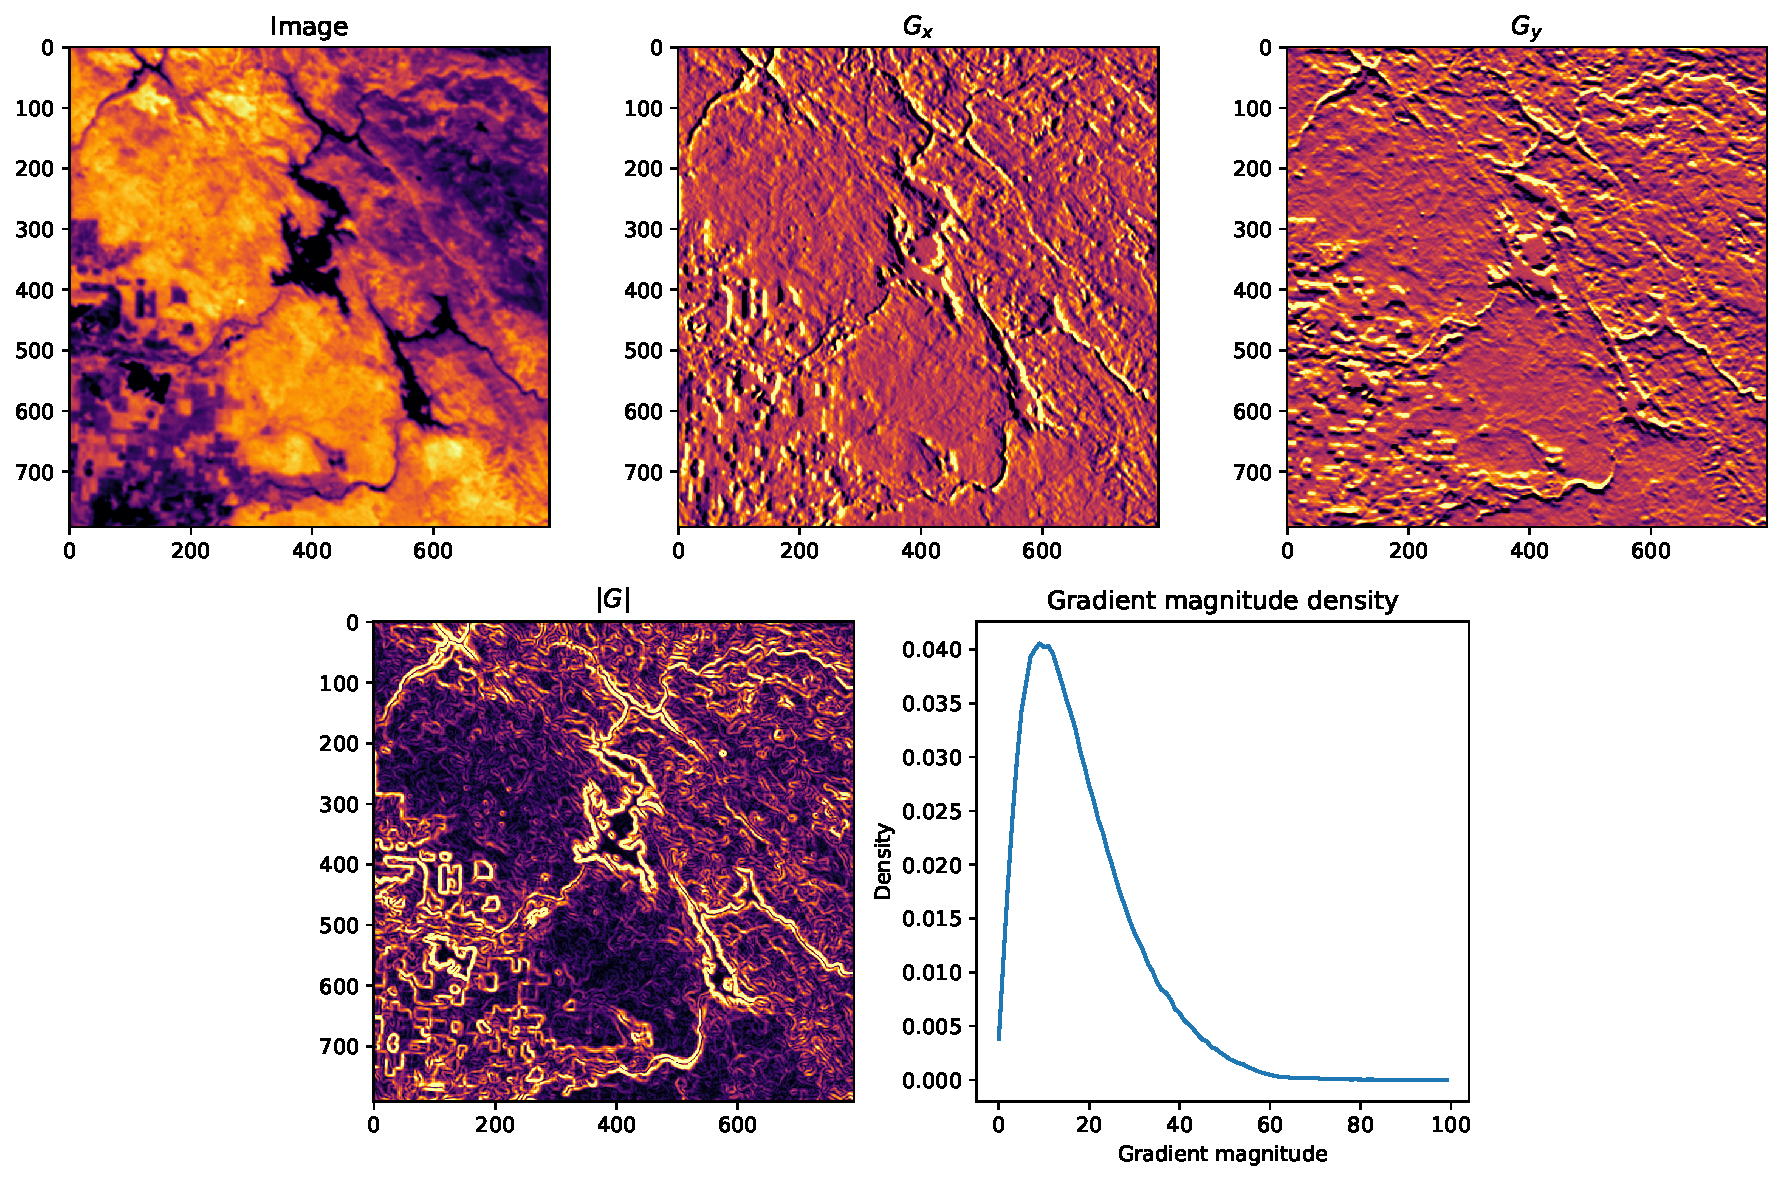
\includegraphics[width=\textwidth]{Includes/4-gradient-analysis.pdf}
             \caption{Steps to obtain a gradient magnitude density. Using the sobel operators, $G_x$ and $G_y$ are obtained from an image. The magnitude $|G|$ of each pixel is calculated using Eq. \ref{eq:4-gradient_magnitude}. The density can be estimated afterwards, using 100 bins in this case.}
             \label{fig:4-gradient-analysis}
         \end{figure}

         

\clearpage

        

        
        
